\documentclass{standalone}
\usepackage{tikz}

\usetikzlibrary{calc}


\begin{document}

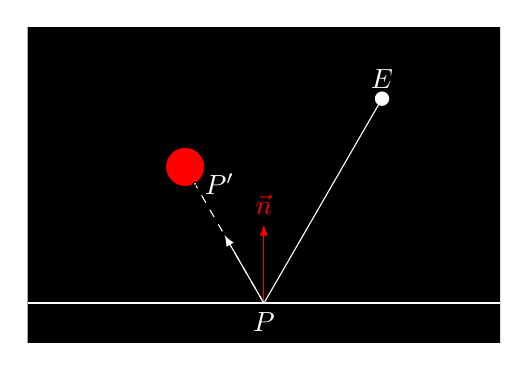
\begin{tikzpicture}
  \path[clip] (-3,-0.5) rectangle (3,3.5);
  \draw[fill=black,black] (-3,-1.5) rectangle (3,3.5);
  \draw[thick,white] (-3,0) -- (3,0);

  \coordinate (hit) at (0,0);
  \coordinate (eye) at (60:3);
  
  \draw[fill=white] (eye) circle [radius=0.1cm] node [white,above] {$E$};
  \node[anchor=north,white] at (hit) {$P$};

  \draw[red,-latex] (hit) -- ++(0,1) node[above] {$\vec n$};

  \draw[white,dashed] (hit) -- ++(120:2);
  \draw[white,-latex] (eye) -- (hit) -- ++(120:1);
  \draw[fill=red] (120:2) circle [radius=0.25cm];
  \draw[fill=white] (120:1.75) circle [radius=0.025cm] node[right,white] {$P'$};
\end{tikzpicture}

\end{document}